\documentclass[tikz]{standalone}

\usepackage{xcolor}

\usetikzlibrary{positioning}

\definecolor{stgoblue}{RGB}{74,144,226}
\definecolor{stgogreen}{RGB}{80,227,194}
\definecolor{stgoorange}{RGB}{255,165,0}
\definecolor{stgored}{RGB}{255,69,0}

\begin{document}

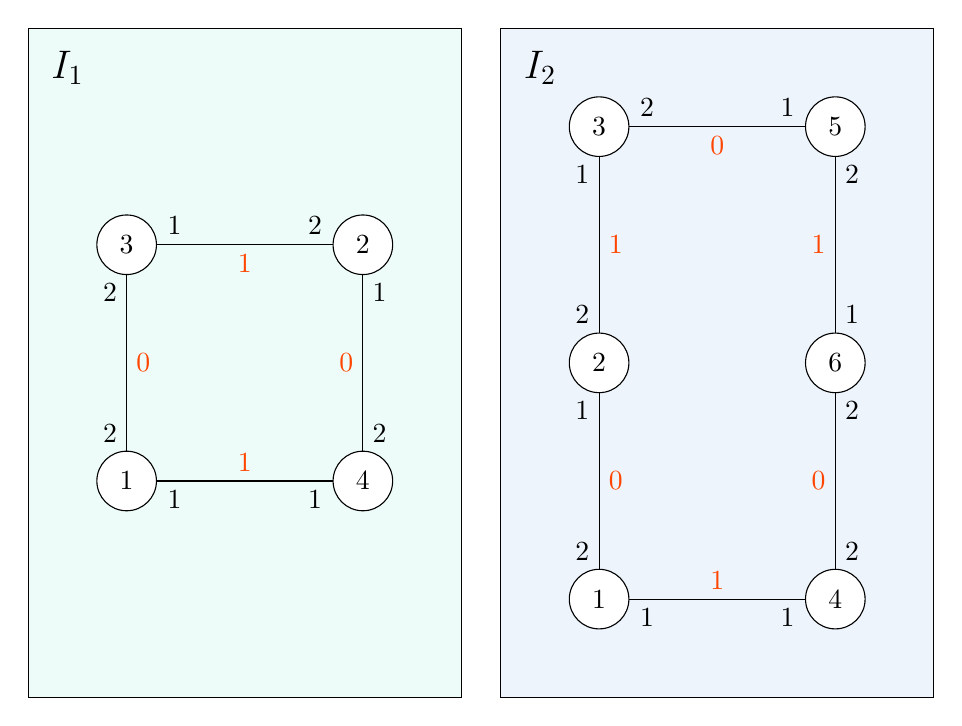
\begin{tikzpicture}
    \tikzstyle{nodeStyle}=[circle, draw, fill=white, inner sep=2pt,
      minimum size=5ex]
    \colorlet{colorLabel}{stgored}
    \tikzstyle{labelStyle}=[draw=none, minimum size=0ex, color=colorLabel]
    \tikzstyle{portStyle}=[labelStyle, color=black]

    \draw[fill=stgogreen!10] (-1.25,2.75) rectangle (4.25,-5.75);
    \node at (-0.75,2.25) {\Large $I_1$};

    %\draw[fill=stgoblue!10] (1,-1.75) rectangle (5,2);
    
    \node[nodeStyle] (3) at (0,0) {$3$};
    \node[nodeStyle] (2) at (3,0) {$2$};
    \node[nodeStyle] (4) at (3,-3) {$4$};
    \node[nodeStyle] (1) at (0,-3) {$1$};

    \draw (3) edge 
      node [pos=0.1,above,portStyle] {$1$}
      node [below,labelStyle] {$1$}
      node [pos=0.9,above,portStyle] {$2$}
    (2);
    \draw (2) edge 
      node [pos=0.1,right,portStyle] {$1$}
      node [left,labelStyle] {$0$}
      node [pos=0.9,right,portStyle] {$2$}
    (4);
    \draw (4) edge 
      node [pos=0.1,below,portStyle] {$1$}
      node [above,labelStyle] {$1$}
      node [pos=0.9,below,portStyle] {$1$}
    (1);
    \draw (1) edge 
      node [pos=0.1,left,portStyle] {$2$}
      node [right,labelStyle] {$0$}
      node [pos=0.9,left,portStyle] {$2$}
    (3);

    \begin{scope}[shift={(6,0)}]
      \draw[fill=stgoblue!10] (-1.25,2.75) rectangle (4.25,-5.75);
      \node at (-0.75,2.25) {\Large $I_2$};

      %\draw[fill=stgoorange!10] (1,-1.75) rectangle (5,2);
    
      \begin{scope}[shift={(0,0.5)}]
        \node[nodeStyle] (4) at (3,-5) {$4$};
        \node[nodeStyle] (1) at (0,-5) {$1$};
        \node[nodeStyle] (2) at (0,-2) {$2$};
        \node[nodeStyle] (3) at (0,1) {$3$};
        \node[nodeStyle] (5) at (3,1) {$5$};
        \node[nodeStyle] (6) at (3,-2) {$6$};
      \end{scope}

      \draw (4) edge 
        node [pos=0.1,below,portStyle] {$1$}
        node [above,labelStyle] {$1$}
        node [pos=0.9,below,portStyle] {$1$}
      (1);
      \draw (1) edge 
        node [pos=0.1,left,portStyle] {$2$}
        node [right,labelStyle] {$0$}
        node [pos=0.9,left,portStyle] {$1$}
      (2);
      \draw (2) edge 
        node [pos=0.1,left,portStyle] {$2$}
        node [right,labelStyle] {$1$}
        node [pos=0.9,left,portStyle] {$1$}
      (3);
      \draw (3) edge 
        node [pos=0.1,above,portStyle] {$2$}
        node [below,labelStyle] {$0$}
        node [pos=0.9,above,portStyle] {$1$}
      (5);
      \draw (5) edge 
        node [pos=0.1,right,portStyle] {$2$}
        node [left,labelStyle] {$1$}
        node [pos=0.9,right,portStyle] {$1$}
      (6);
      \draw (6) edge 
        node [pos=0.1,right,portStyle] {$2$}
        node [left,labelStyle] {$0$}
        node [pos=0.9,right,portStyle] {$2$}
      (4);
    \end{scope}
\end{tikzpicture}

\end{document}
